\documentclass{cours}
\usepackage{pgfplots}
\usepackage{amssymb}
\usepackage[version=4]{mhchem}
\usepackage{chemfig}
\DeclareMathOperator{\NO}{n.o.}
\begin{document}

\setcounter{chapter}{15}
\chapter{Oxydoréduction}
\section{Oxydant et réducteur}%
\label{sec:oxydant_et_reducteur}

\subsection{Couple oxydant/réducteur}%
\label{sub:couple_oxydant_reducteur}

Un couple oxydant/réducteur est un couple de deux espèces d'un même élément chimique.
\begin{itemize}
  \item L'oxydant doit \textbf{capter} un ou plusieurs électrons pour se transformer en réducteur (réduction);
  \item Le réducteur doit \textbf{céder} un ou plusieurs électrons pour se transformer en oxydant (oxydation);
\end{itemize}

Par exemple, pour le couple \ce{Cu^2+ (aq)/Cu(s)} on a 
\begin{equation}
  \ce{Cu^2+ + 2e- <=> Cu(s)}
\end{equation}
dans ce cas, \ce{Cu^2+(aq)} est l'oxydant et \ce{Cu(s)} est le réducteur.

Pour le couple \ce{Br2(aq)}/\ce{Br-(aq)} on a 
\begin{equation}
  \ce{Br2(aq) + 2e- <=> 2Br-(aq)}
\end{equation}
dans ce cas, \ce{Br2(aq)} est l'oxydant et \ce{Br-(aq)} est le réducteur. 

Les réactions d'oxydo-réduction ne faisant en milieu aqueux, la demi-équation associée au couple peut faire intervenir \ce{H+} et \ce{H2O}. Par exemple pour le couple \ce{IO3-}/\ce{I2} on a 
\begin{equation}
  \ce{IO3- + 6H+ +5e- <=> \frac{1}{2}I2 + 3H2O}
\end{equation}

Les espèces suivantes sont à connaître :
\begin{center}
  \begin{tabular}{llll}
  \toprule
  Nom & Formule & Nature & Couple \\
  \midrule
  thiosulfate & \ce{S2O3^2-}& réducteur & \ce{S4O6^2-/S2O3^2-} \\
  permanganate & \ce{MnO4^-} & oxydant  & \ce{MnO4^-/Mn^2+}\\
  hypochlorite & \ce{ClO-}& oxydant & \ce{ClO^-/Cl-}\\
  peroxyde d'hydrogène & \ce{H2O2}& oxydant & \ce{H2O2/H2O}\\
  \bottomrule
    
  \end{tabular}
\end{center}

\subsection{Nombre d'oxydation}%
\label{sub:nombre_d_oxydation}

Pour caractériser le \emph{degré d'oxydation} d'un élément chimique, on lui associe un \textbf{nombre d'oxydation}. Le nombre d'oxydation correspond à la charge que porterait l'élément si les électrons de chaque liaison étaient captés par l'atome le plus électronégatif de la liaison.

En général, on écrit les nombres d'oxydation en chiffres romains (I, II, III, IV, V, VI, VII).

La somme des nombres d'oxydation des atomes qui forment une molécule ou un ion est égale à la charge totale portée par l'ion ($0$ pour une molécule non chargée).
Par exemple 
\begin{itemize}
  \item Dans \ce{MnO4-} : $\NO(\ce{Mn})+4\NO(\ce{O}) = -\text{I}$ ;
  \item dans \ce{CO2} : $\NO(\ce{C}) + 2\NO(\ce{O}) = 0$ ;
  \item dans \ce{I2} : $\NO(\ce{I}) = 0$ .
\end{itemize}

Très souvent, dans une molécule composée, on aura $\NO(\ce{O})=-\text{II}$ et $\NO(\ce{H})=\text{I}$. Mais ça n'est pas toujours le cas, par exemple dans \ce{O2}, $\NO(\ce{O})=\text{0}$.

Parfois, différents atomes d'un même élément chimique n'ont pas le même nombre d'oxydation au sein d'une molécule. Par exemple dans l'ion thiosulfate :
\begin{center}
   \chemfig{
   S
   (=[:-45]\charge{0=\|,-90=\|}{O})
   (=\charge{45=\|, -45=\|}{S})
   (-[:90] \charge{0=\|, 90=\|, 180=\|, 45:4pt=$\scriptstyle\ominus$}{O})
   (-[:225] \charge{-45=\|, -135=\|, -225=\|, 90:4pt=$\scriptstyle\ominus$}{O})
   } 
\end{center}
l'atome de soufre central à un nombre d'oxydation de +IV alors que l'atome de soufre périphérique a un nombre d'oxydation de 0. 

Pour connaître de manière certaine le nombre d'oxydation d'un atome dans une molécule, il faut connaitre la structure de la molécule.

La position d'un atome dans la classification périodique permet de connaître ses degrés d'oxydation extrêmes. En effet, un atome ne peut pas perdre plus d'électrons que son nombre d'électrons de valence et ne peut pas capter plus d'électrons que le nombre nécessaire à saturer sa couche de valence.

Par exemple l'atome d'oxygène \ce{_8O} a la configuration électronique :
\begin{equation}
  1s^2 2s^2 2p^4
\end{equation}
possède 6 électrons de valence, on pourra le trouver avec un nombre d'oxydation compris entre -II (il gagne deux électrons et remplit sa sous-couche $2p$) et +VI (il perd tous ses électrons de valence). 

En pratique on rencontre très rarement l'oxygène avec un nombre d'oxydation positif. Pour cela, il faudrait qu'il forme une molécule avec un élément plus électronégatif que lui, ce qui est très rare (c'est le cas seulement dans la molécule de \ce{OF2}).

\subsection{Pile}%
\label{sub:pile}

Une \textbf{demi-pile} correspond à la mise en contact d'un oxydant avec le réducteur associé, en général l'un des deux est solide et l'autre est en solution aqueuse.

Par exemple, on plonge un morceau de zinc solide dans une solution de sulfate de zinc

\begin{center}
  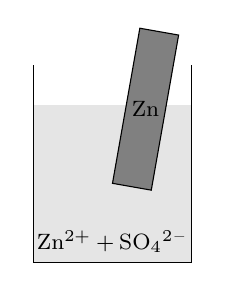
\begin{tikzpicture}
  %tikz redox
    \fill[gray!20] (0,0) rectangle (2,2);
    \draw (0,2.5) -- (0,0) -- node[above]{\footnotesize\ce{Zn^2+ + SO4^2-}}(2, 0) -- (2, 2.5);
    \draw[fill=gray, rotate around={-10:(1,1)}] (1,1) rectangle (1.5, 3) (1.25,2) node{\footnotesize Zn};
  \end{tikzpicture}
  \captionof{figure}{Demi-pile du couple \ce{Zn^2+/Zn}}
\end{center}

On forme une \textbf{pile} en reliant deux demi-piles par un \textbf{pont salin} qui permet la circulation des ions. Le pont salin peut être constitué d'une solution ionique gélifiée. 

\begin{center}
  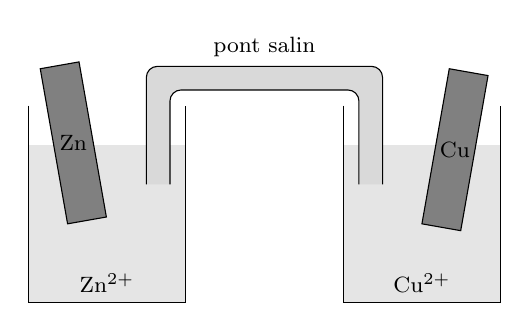
\begin{tikzpicture}
  %tikz redox
    \fill[gray!20] (0,0) rectangle (2,2);
    \draw (0,2.5) -- (0,0) -- node[above]{\footnotesize\ce{Zn^2+}}(2, 0) -- (2, 2.5);
    \draw[fill=gray, rotate around={10:(0.5,1)}] (0.5,1) rectangle (1, 3) (0.75,2) node{\footnotesize Zn};
    \begin{scope}[xshift=4cm]
    \fill[gray!20] (0,0) rectangle (2,2);
    \draw (0,2.5) -- (0,0) -- node[above]{\footnotesize\ce{Cu^2+}}(2, 0) -- (2, 2.5);
    \draw[fill=gray, rotate around={-10:(1,1)}] (1,1) rectangle (1.5, 3) (1.25,2) node{\footnotesize Cu};
    \end{scope}
    \fill[gray!30] (1.5, 1.5) [rounded corners]-- (1.5, 3) -- (4.5, 3) [sharp corners]-- (4.5, 1.5) -- (4.2, 1.5) [rounded corners]-- (4.2, 2.7)-- (1.8, 2.7) --(1.8, 1.5);
    \draw[rounded corners] (1.5, 1.5) -- (1.5, 3) --node[above]{\footnotesize pont salin} (4.5, 3) -- (4.5, 1.5);
    \draw[rounded corners] (1.8, 1.5) -- (1.8, 2.7) -- (4.2, 2.7) -- (4.2, 1.5);
  \end{tikzpicture}
  \captionof{figure}{Pile des couples \ce{Zn^2+/Zn} et \ce{Cu^2+/Cu}}
\end{center}
\newcommand{\sslash}{\mathbin{/\mkern-4mu/}}
On symbolise cette pile par \ce{Zn^2+/Zn \sslash Cu^2+/Cu}


Lorsqu'on relie les deux électrodes par un voltmètre de grande impédance d'entrée, il indique une tension 
\begin{equation}
  U = V_{\ce{Cu}} - V_{\ce{Zn}} \approx \SI{1.1}{\volt}
\end{equation}
Cette tension s'appelle \textbf{tension à vide}  (ou \textbf{force électromotrice}, fem) de la pile. Dans ce cas, $V_{\ce{Cu}}>V_{\ce{Zn}}$, \ce{Cu} est l'électrode positive (cathode) et \ce{Zn} est l'électrode négative (anode)

Les atomes de zinc fournissent des électrons au circuit extérieur, donc il se produit une oxydation
\begin{equation}
  \ce{Zn -> Zn^2+ + 2e^-}
\end{equation}


L'électrode de  cuivre capte des électrons, il s'y produit donc une réduction :
\begin{equation}
  \ce{Cu^2+ + 2e- -> Cu}
\end{equation}

Le bilan global de la réaction qui se produit au sein de la pile est :
\begin{equation}
  \ce{Cu^2+ + Zn -> Cu + Zn^2+}
\end{equation}

\subsection{Potentiel d'électrode}%
\label{sub:potentiel_d_electrode}

Une pile ne permet de définir qu'une différence de potentiel entre deux couples. Pour fixer l'origine des potentiels, on utilise l'électrode standard à hydrogène (ESH)  

\begin{center}
  \begin{tikzpicture}
  %tikz redox
    
    \fill[gray!20] (0,0) rectangle (2,2);
    \draw (0,2.5) -- (0,0) -- (2, 0) -- (2, 2.5);
    \draw[fill=white] (-1, 3) -- (0.3, 3) -- (0.3,0.5) --(1.5,0.5) -- (1.5, 0.7) -- (0.5, 0.7) -- (0.5, 3.2) -- (-1, 3.2);
    \draw [latex-] (-1, 3.1) -- ++(-1,0) node[left]{$p_{\ce{H2}}=\SI{1}{\bar}$}; 
    \draw (1.8, 0.2) -- ++(1,0.5) node[right]{$a_{\ce{H3O+}}=1$ };
    \foreach \i in {1,2,...,20}{
      %\pgfmathsetmacro{\x}{0.6+random*0.8}
      %\pgfmathsetmacro{\y}{0.75+random*1.1}
      \draw[fill=white]({0.6+abs(rand)*0.8}, {0.75+abs(rand)*1.1}) circle(0.05);
    }
    \draw[thick] (3, 3) node[right]{électrode de platine} -- (1.7, 3) -- (1.7, 1) ;
    \draw[thick,decorate,
    decoration={coil, segment length=3pt}]
    (1.7,1)-- (0.7, 1);
  \end{tikzpicture}
  \captionof{figure}{Électrode standard à hydrogène}
\end{center}

La demi-équation de cette demi-pile est 
\begin{equation}
  \ce{2H3O+(aq) + 2e- <=> H2(g) + 2H2O(l)}
\end{equation}

Et par convention son potentiel est pris égal à \SI{0}{\volt}. Le \textbf{potentiel standard} $E^\circ_{\ce{Ox/Red}}$  d'un couple oxydant/réducteur est déterminé en réalisant une pile comportant une ESH et une électrode associant les deux espèces du couple avec toutes les activités égales à 1.

\subsection{Formule de Nernst}%
\label{sub:formule_de_nernst}

La formule de Nernst donne le potentiel $E_{\ce{Ox}/\ce{Red}}$ d'un couple \ce{Ox}/\ce{Red} en fonction de de son potentiel standard $E^\circ_{\ce{Ox/Red}}$ et des caractéristiques physiques des espèces de la demi-équation associée au couple.

\begin{loi}{Formule de Nernst}
Le potentiel du couple de demi-équation 
\begin{equation}
  \nu_O\ce{Ox} + \sum_i \nu_i \ce{A_i} + \ce{ne-} \ce{<=>} \nu_R \ce{Red} + \sum_j \nu_j \ce{B_j}
\end{equation}
est donné par 
\begin{equation}
  E_{\ce{Ox/Red}} = E^\circ_{\ce{Ox/Red}} + \frac{RT}{n\mathcal{F}} \ln \left( \frac{a_{\ce{Ox}}^{\nu_O}\prod_i a_{\ce{A_i}}^{\nu_i}}{a_{\ce{Red}}^{\nu_R}\prod_j a_{\ce{B_j}}^{\nu_j}} \right)
\end{equation}
avec
\begin{itemize}
  \item $\mathcal{F}=\SI{96485}{\coulomb\per\mole}$ la constante de Faraday ;
  \item $R$ la constante des gaz parfaits.
\end{itemize}
\end{loi}

On notera que lorsque $T=\SI{25}{\celsius}$ on a $\frac{RT}{\mathcal{F}}\ln(x)\approx \num{0.06}\log(x)$, donc à cette température, on pourra utiliser l'expression suivante de la formule de Nernst :
\begin{equation}
  E_{\ce{Ox/Red}} = E^\circ_{\ce{Ox/Red}} + \frac{0.06}{n} \log \left( \frac{a_{\ce{Ox}}^{\nu_O}\prod_i a_{\ce{A_i}}^{\nu_i}}{a_{\ce{Red}}^{\nu_R}\prod_j a_{\ce{B_j}}^{\nu_j}} \right)
\end{equation}

Par exemple, pour le couple \ce{CU^2+/Cu} de demi-équation 
\begin{equation}
  \ce{Cu^2+(aq) + 2e- <=> Cu(s)}
\end{equation}
on a 
\begin{equation}
  E_{\ce{Cu^2+/Cu}} =  E^\circ_{\ce{Cu^2+/Cu}} + \frac{RT}{2\mathcal{F}}\ln \left( \frac{[\ce{Cu^2+}]}{\cz} \right)
\end{equation}

Et pour le couple \ce{Cr2O7^2-/Cr^3+} de demi-équation 
\begin{equation}
  \ce{Cr2O7^2- + 14H+ + 6e- <=> 2Cr^3+ + 7H2O}
\end{equation}
on a
\begin{equation}
  E = E^\circ + \frac{RT}{6\mathcal{F}} \ln \left( \frac{[\ce{H+}]^{14}[\ce{Cr2O7^2-}]}{\cz^{13} [\ce{Cr^3+]^2}} \right)
\end{equation}

\subsection{Diagramme de prédominance}%
\label{sub:diagramme_de_predominance}
Considérons le couple \ce{Fe^3+/Fe^2+}, de demi-équation \ce{Fe^3+ + e- <=> Fe^2+}, le potentiel d'une solution contenant des ions \ce{Fe^3+} et des ions \ce{Fe^3+} à \SI{25}{\celsius} est donné par
\begin{equation}
  E_{\ce{Fe^3+/Fe^2+}} = E^\circ_{\ce{Fe^3+/Fe^2+}} + \num{0.06} \log \left(\frac{[\ce{Fe^3+]}}{[\ce{Fe^2+}]}\right)
\end{equation} 

Dans ces conditions :
\begin{itemize}
  \item Si $[\ce{Fe^3+}]>[\ce{Fe^2+}]$ alors $E>E^\circ$ et \ce{Fe^3+} est prédominant en solution ;   
  \item Si $[\ce{Fe^2+}]>[\ce{Fe^3+}]$ alors $E<E^\circ$ et \ce{Fe^2+} est prédominant en solution ;   
\end{itemize}

On peut dresser le diagramme de prédominance :
\begin{center}
  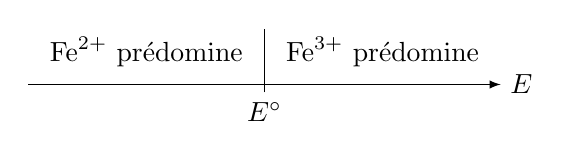
\begin{tikzpicture}
  %tikz redox
    \draw[-latex] (0,0) -- (6, 0) node[right] {$E$ };
    \draw (3,-0.1) node[below]{$E^\circ$} -- (3, 0.7);
    \draw (1.5, 0.1) node[above]{\ce{Fe^2+} prédomine};
    \draw (4.5, 0.1) node[above]{\ce{Fe^3+} prédomine};
  \end{tikzpicture}
\end{center}




\section{Réaction d'oxydo-réduction}%
\label{sec:reaction_d_oxydo_reduction}

\subsection{Prévision qualitative}%
\label{sub:prevision_qualitative}
Le potentiel d'une solution a une valeur bien définie. Si on met en solution deux espèces dont les domaines de prédominance ne se superposent pas, il n'existe pas de potentiel qui permette que ces deux espèces restent prédominantes, elles vont réagir entre elles.

Lorsque l'on met deux couples oxydant/réducteur en solution, on peut prévoir qualitativement le sens dans lequel va se produire la réaction par la \emph{règle du gamma} :

\begin{center}
  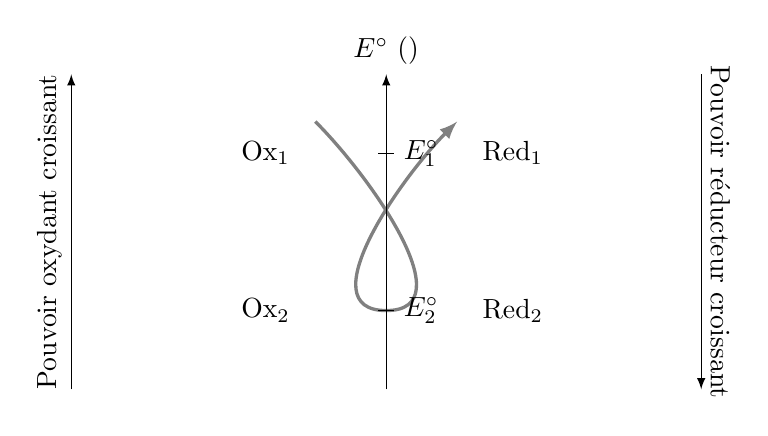
\begin{tikzpicture}
  %tikz redox
    \draw[very thick, gray, -latex] (-0.9, 3.4) to[out=-45, in=0] (0, 1) to[out=180, in=-135] (0.9, 3.4);
    \draw[-latex] (-4,0) -- (-4, 4) node[midway, rotate=90, above]{Pouvoir oxydant croissant};
    \draw[latex-] (4,0) -- (4, 4) node[midway, rotate=-90, above]{Pouvoir réducteur croissant};
    \draw[-latex] (0,0) -- (0,4) node[above]{$E^\circ$ (\si{\volt})}; 
    \draw (-0.1, 1) node[left, xshift=-1cm]{\ce{Ox2}} -- (0.1, 1) node[right]{$E^\circ_2$} node[right, xshift=1cm]{\ce{Red2}};
    \draw (-0.1, 3) node[left, xshift=-1cm]{\ce{Ox1}} -- (0.1, 3) node[right]{$E^\circ_1$} node[right, xshift=1cm]{\ce{Red1}};
  \end{tikzpicture}
\end{center}

La réaction a lieu entre l'oxydant le plus fort (\ce{Ox1}) et le réducteur le plus fort (\ce{Red2}).

Par exemple, pour les couples
\begin{itemize}
  \item \ce{MnO4^-/Mn^2+}, $E^\circ_1= \SI{1.51}{\volt} $, demi-équation : \ce{MnO4- + 8H+ +5e- <=> Mn^2+ + 4H2O}
  \item \ce{Fe^3+/Fe^2+}, $E^\circ_2= \SI{0.77}{\volt} $, demi-équation : \ce{Fe^3+ + e- <=> Fe^2+}
\end{itemize}

On a 
\begin{center}
  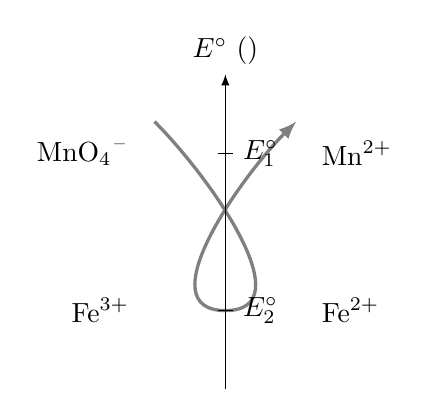
\begin{tikzpicture}
  %tikz redox
    \draw[very thick, gray, -latex] (-0.9, 3.4) to[out=-45, in=0] (0, 1) to[out=180, in=-135] (0.9, 3.4);
    \draw[-latex] (0,0) -- (0,4) node[above]{$E^\circ$ (\si{\volt})}; 
    \draw (-0.1, 1) node[left, xshift=-1cm]{\ce{Fe^3+}} -- (0.1, 1) node[right]{$E^\circ_2$} node[right, xshift=1cm]{\ce{Fe^2+}};
    \draw (-0.1, 3) node[left, xshift=-1cm]{\ce{MnO4-}} -- (0.1, 3) node[right]{$E^\circ_1$} node[right, xshift=1cm]{\ce{Mn^2+}};
  \end{tikzpicture}
\end{center}
et il se produit la réaction
\begin{equation}
  \ce{8H+ + MnO4- + 5Fe^2+ -> Mn^2+ + 4H2O + 5Fe^3+}
\end{equation}
\subsection{Constante d'équilibre}%
\label{sub:constante_d_equilibre}
Considérons deux couples de demi-équations 
\begin{align}
  & \ce{Ox1 + $n_1$ e- <=> Red1}\\
  & \ce{Ox2 + $n_2$ e- <=> Red2}
\end{align}
La réaction entre \ce{Ox1} et \ce{Red2} a pour équation
\begin{equation}
  \ce{$n_2$Ox_1 + $n_1$Red2 <=> $n_1$Ox2 + $n_2$ Red1}
\end{equation}
Et sa constante d'équilibre s'écrit :
\begin{equation}
  K = \frac{a(\ce{Ox2})^{n_1}a(\ce{Red1})^{n_2}}{a(\ce{Ox1})^{n_2}a(\ce{Red2})^{n_1}}
\end{equation}
Comme les deux couples partagent la même solution, leurs potentiels doivent être égaux à l'équilibre et la formule de Nernst donne 
\begin{equation}
  E^\circ_1 + \frac{RT}{n_1\mathcal{F}}\ln \left( \frac{a(\ce{Ox1})}{a(\ce{Red1})} \right) =  E^\circ_2 + \frac{RT}{n_2\mathcal{F}}\ln \left( \frac{a(\ce{Ox2})}{a(\ce{Red2})} \right)
\end{equation}
ce qui donne 
\begin{equation}
  E^\circ_1-E^\circ_2 = \frac{RT}{n_1n_2\mathcal{F}}\ln(K)
\end{equation}
et donc finalement 
\begin{eqencadre}
  K = \exp \left( \frac{n\mathcal{F}}{RT} (E^\circ_1-E^\circ_2) \right)
\end{eqencadre}
avec $n=n_1n_2$. 

À \SI{25}{\celsius}, cette relation peut s'écrire :
\begin{equation}
\large
  K = 10^{\frac{n}{0.06}(E^\circ_1-E^\circ_2)}
\end{equation}

\subsection{Dismutation et médiamutation}%
\label{sub:dismutation_et_mediamutation}
Il peut arriver qu'une même espèce chimique intervienne dans plusieurs couples. Dans ce cas il peut se produire une \textbf{dismutation}. Par exemple le peroxyde d'hydrogène (eau oxygénée) intervient dans les couples suivants :

\begin{center}
  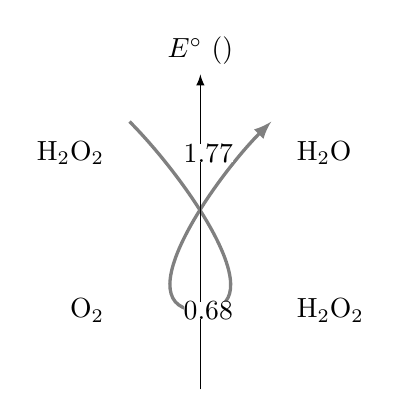
\begin{tikzpicture}
  %tikz redox
    \draw[very thick, gray, -latex] (-0.9, 3.4) to[out=-45, in=0] (0, 1) to[out=180, in=-135] (0.9, 3.4);
    \draw[-latex] (0,0) -- (0,4) node[above]{$E^\circ$ (\si{\volt})}; 
    \draw (-0.1, 3) node[left, xshift=-1cm]{\ce{H2O2}} -- (0.1, 3) node[fill=white, inner sep=0]{ \SI{1.77}{\volt} } node[right, xshift=1cm]{\ce{H2O}};
    \draw (-0.1, 1) node[left, xshift=-1cm]{\ce{O2}} -- (0.1, 1) node[fill=white, inner sep=0]{ \SI{0.68}{\volt}} node[right, xshift=1cm]{\ce{H2O2}};
  \end{tikzpicture}
\end{center}

Le bilan de cette réaction est 
\begin{equation}
  \underbrace{\ce{2H2O2}}_{-\text{I}} \ce{<=>} \underbrace{\ce{O2}}_{0} + \underbrace{\ce{2H2O}}_{-\text{II}}
\end{equation}

On remarque qu'on part d'une espèce chimique dans laquelle l'oxygène a un nombre d'oxydation de $-\text{I}$ et on obtient deux espèces chimiques, l'une avec un nombre d'oxydation plus grand et l'autre avec un nombre d'oxydation plus faible. 

On peut également voir une \textbf{médiamutation} au cours de laquelle deux espèces chimiques réagissent pour en donner une seul de nombre d'oxydation intermédiaire. Par exemple  

\begin{center}
  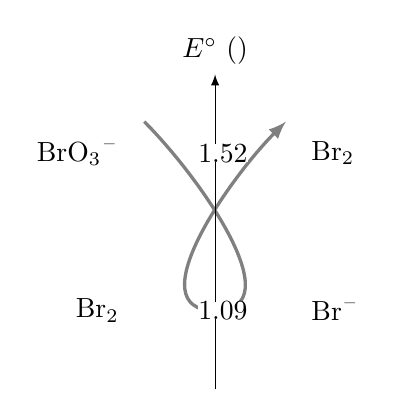
\begin{tikzpicture}
  %tikz redox
    \draw[very thick, gray, -latex] (-0.9, 3.4) to[out=-45, in=0] (0, 1) to[out=180, in=-135] (0.9, 3.4);
    \draw[-latex] (0,0) -- (0,4) node[above]{$E^\circ$ (\si{\volt})}; 
    \draw (-0.1, 3) node[left, xshift=-1cm]{\ce{BrO3-}} -- (0.1, 3) node[fill=white, inner sep=0]{ \SI{1.52}{\volt} } node[right, xshift=1cm]{\ce{Br2}};
    \draw (-0.1, 1) node[left, xshift=-1cm]{\ce{Br2}} -- (0.1, 1) node[fill=white, inner sep=0]{ \SI{1.09}{\volt}} node[right, xshift=1cm]{\ce{Br-}};
  \end{tikzpicture}
\end{center}
dont l'équation bilan est :
\begin{equation}
  \underbrace{\ce{2BrO3-}}_{\text{V}} + \ce{12H+} + \underbrace{\ce{10Br-}}_{-\text{I}} \ce{<=>} \underbrace{\ce{6Br2}}_{0} + \ce{6H2O}
\end{equation}
\end{document}
